\chapter{Photometry}

\label{ch_photometry}

% This chapter describes the methods used to obtain the observational data as well as the methods used to clean, prepare and analyse the datasets.
% 
% For this project measurements of the object's brightness were taken simultaneously with its spectrum. Both the photometric and spectroscopic  measurements were obtained using short exposure times in order to have high time resolution.

\section{SAAO 1.9m Radcliff Reflector}

\label{saao1.9}

The photometric observations were made using the 1.9m reflector at the SAAO (South African Astronomical Observatory) site in Sutherland. The telescope was built during 1938 to 1948 by Grubb-Parsons. It was originally situated at the Radcliff Observatory outside Pretoria, but was moved to Sutherland in the seventies due to bad light pollution in Pretoria.

The telescope is equatorially mounted, and is used in a Cassegrain configuration at the f/18 focus. It can be fitted with a variety of instruments, the most common being the UCT CCD photometer, a grating spectrograph and a fibre fed Echelle spectrograph.

Details of this telescope can be found at http://www.saao.ac.za/.

\section{UCT CCD Photometer}
\label{uctccd}

The UCT CCD photometer is a Wright Instruments Peltier cooled camera. It has a 576x420 thinned, back illuminated EEV CCD. The instrument can be used on the 1.9m,1.0m and 0.75m telescopes at Sutherland. The instrument is controlled by a 486 computer running MS-DOS \citep{UCTCCD}.

It can be used in various configurations. The gain can be set depending on the brightness of the target objects. The gain is the ratio of photo-electrons to Analog-to-Digital units (ADU). The gain can be set to either 1 or 4. Gain 1 corresponds to 10 photo-electrons/ADU and gain 4 corresponds to 2.5 photo-electrons/ADU. This option is available to optimise signal-to-noise ratios for bright and faint stars. With the gain set to 1, a higher number of photo-electrons can be read before the analog-to-digital converter saturates. This setting is used for bright stars. On gain set to 4, a higher number of ADUs are read per photo-electron thereby decreasing the noise added by the readout process.  The gain was set to 4 for all the observations made for this project.

The CCD can be prebinned before the values are read out, in order to reduce readout noise and increase the signal-to-noise ratio. The instrument allows prebinning values from 1x1 to 6x6. However, using too much binning may result in stellar images that are undersampled for precise PSF fitting. A general rule of thumb is to  select the prebinning such that the star occupies $\sim$2.2 pixels on the output image. The image scale is 0.139 arcsec/pixel on the 1.9m telescope and generally prebinning values of 3x3 or greater are used, depending on seeing conditions.

The CCD is also equipped to perform observations in frame transfer mode. In this mode, half the CCD is masked by a frame transfer mask. The unmasked half is then exposed, after which the counts are transferred to the masked half of the CCD where they can be read out while the unmasked area is exposed again. This minimises the downtime between exposures. This high-speed mode was used for the observations made for this project.




\section{Photometric Observations}
\label{sub_observations}
Photometric observations of EC2117-54 were made on 4 consecutive nights during 16 to 19 August 2006. The runs on 18 and 19 August were hampered by cloud.  The observations were made using a Johnson V filter in order to provide a way of correlating the photometric and spectroscopic observations. An integration time of 6 seconds was selected. This is the highest time resolution that is reliable on this instrument and is well within the Nyquist frequency for the most rapid oscillations that were to be studied.  The shortest timescale of the variations under study is approximately 20 seconds. The telescope was pointed in such a way to ensure that the image contained at least one relatively bright non-variable star that can be used to calculate differential corrections (Figure \ref{exposure}).

See table \ref{obslog} for the full observation log.

\begin{table}
\begin{scriptsize}
\centering
% use packages: array
\begin{tabular}{ccccccccc}
\hline\hline\\Object & Type & Run No & Date            & HJD of first obs & Length & $t_{in}$ & Tel & Filter \\ 
                     &      &        &(start of night) &     (+2453900)   &    (h)   & (s) &       & \\\\ \hline  \\
	EC2117       & NL   & S7651  & 16 Aug 2006     &    64.28141      &  5.35    & 6s  & 74-in & V \\ 
	EC2117       & NL   & S7655* & 17 Aug 2006     &    65.32565      &  6.26    & 6s  & 74-in & V \\  
        EC2117       & NL   & S7659  & 18 Aug 2006     &    66.31921      &  4.36    & 6s  & 74-in & V \\ 
        EC2117       & NL   & S7661  & 19 Aug 2006     &    67.40985      &  0.74    & 6s  & 74-in & V \\\\ \hline \\

\end{tabular}
Notes: NL = Nova-like, $t_{in}$ = integration time, V = Johnson V, * = Simultaneous observations with SALT time-resolved spectroscopy, All observations made with UCT CCD.
\end{scriptsize}
\caption[Photometric Observations Log]{Photometric Observations Log}
\label{obslog}
\end{table}





\section{Reduction of Photometric Measurements}

\label{phot_reductions}

The images obtained from the UCT CCD photometer are stored on a computer separate from the guide computer and the instrument's computer. They are stored in the widely used FITS (Flexible Image Transportation System) format. Before the stellar brightnesses can be measured, the images must be corrected for systematic errors. These include the non-uniform quantum efficiency of the individual pixels, dust on the CCD and filters, cosmic ray hits, dark current and bias.

The exposures are cleaned, calibrated and reduced using a program written by Darragh O'Donoghue. These are available on the computers at Sutherland and are used to reduce exposures ``on-the-fly'' at the telescope. The flatfields are created using the program `cleen'. The stellar brightnesses are extracted using the program 'reduce'. The differential corrections are applied using the program `diffphot'.

The images have been been corrected by dividing them with a master flatfield image. A master flatfield image is constructed by taking images of the twilight sky before any stars become visible. The twilight sky is essentially of uniform brightness over the field of view of the telescope. The telescope is set to point in the same direction during these exposures. This will ensure that bright stars leave a trail on an image. A large number of these images are used by calculating the median for every pixel over all the flatfield exposures. This ensures that any cosmic ray hits and stellar trails will be discarded.

CCD chips are given an initial amount of electrons in the pixels to avoid having a negative value when the pixels are read out. This is called the bias. This is corrected by measuring the bias value on the overscan strip that are read out when the image is read out by the instrument. This measured value is then subtracted from the entire image.


After the images have been cleaned and calibrated, the stellar brightnesses must be measured. This is generally done in one of two ways. The most common way is to use the aperture magnitude method. This method uses an annulus centred on a star. The radius of the annulus is chosen such that the inner circle contains the entire stellar image, and the annulus contains only the sky background. The counts inside the background annulus is then added up and the average per pixel is calculated, which is then subtracted from every pixel inside the inner circle. The pixel values in this circle is then added up. This gives a measure of the brightness of the star.

The second method used is that of Point Spread Function (PSF) fitting. A PSF is a mathematical function which represents the distribution of light across a stellar image. The PSF model is fitted to the brightest stars on an image, and are then scaled for every individual star. This ensures that the shape of the PSF is modelled on a high signal-to-noise ratio image. The scaled PSF's are then integrated to produce measures of stellar brightnesses.

The differentially corrected lightcurves are shown in Figure \ref{lightcurves}. They are displayed in order from top to bottom and are vertically displaced by arbitrary amounts for display purposes. The eclipses can be seen clearly in the lightcurves. Also note the random variations in the lightcurves out of eclipse.

\begin{figure}
\begin{center}
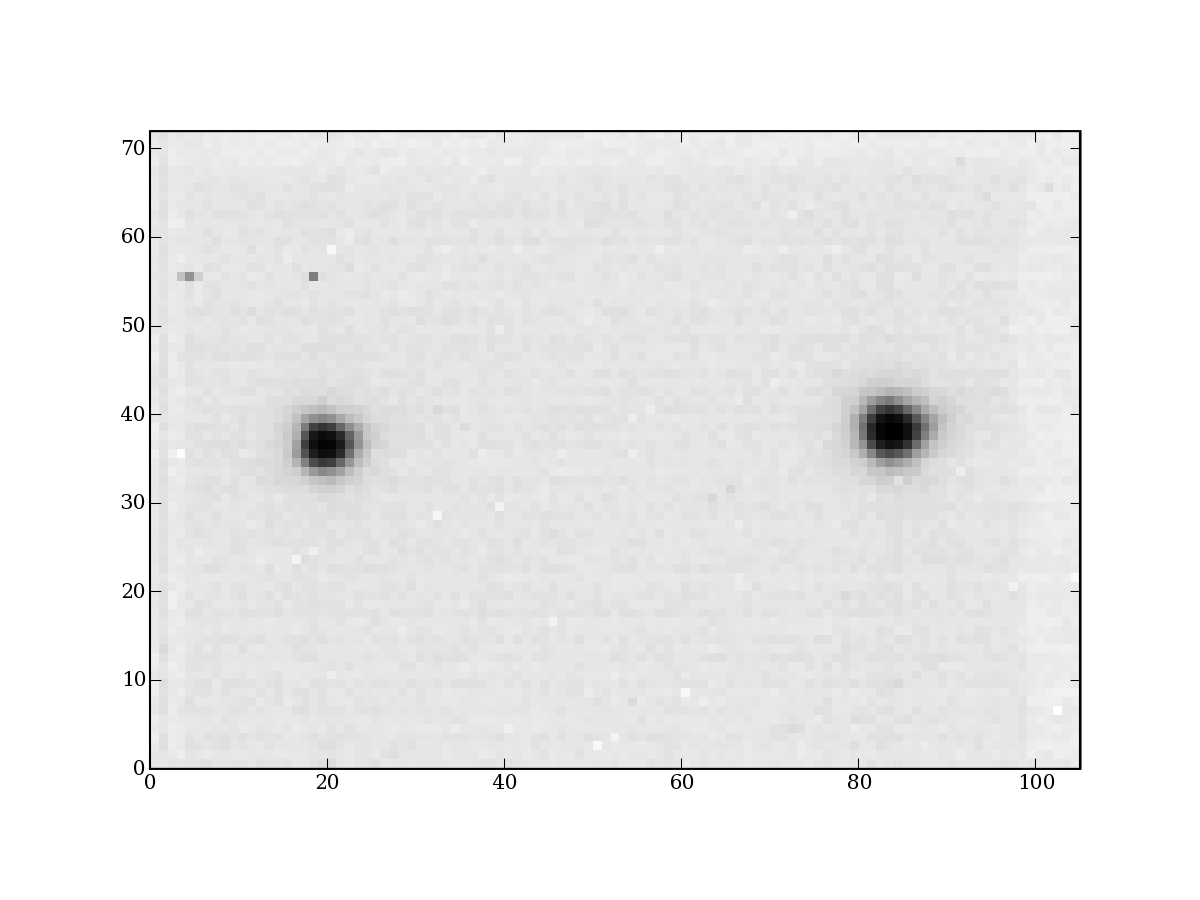
\includegraphics[bb=0 0 600 400,width=0.85\columnwidth]{images/inv_exposure.png}
% ec2117fits.png: 600x400 pixel, 72dpi, 21.17x14.11 cm, bb=0 0 600 400
\caption[Example of photometric exposure]{Example of photometric exposure of EC2117-54 and comparison star.}
\label{exposure} 
\end{center}
\end{figure}


\begin{figure}
\begin{center}
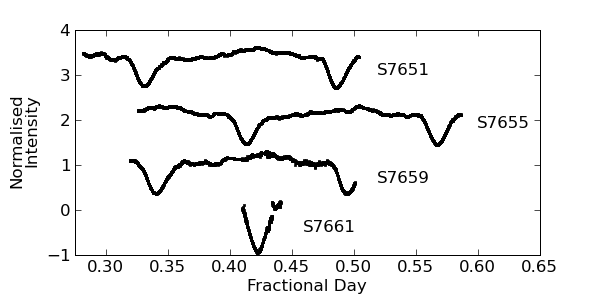
\includegraphics[bb=0 0 600 400,width=0.85\columnwidth]{images/lightcurves.png}
 % lightcurves.png: 600x400 pixel, 72dpi, 21.17x14.11 cm, bb=0 0 600 400
\caption[Lightcurves of EC2117 for 16-19 August 2006.]{Lightcurves of EC2117 for 16-19 August 2006. They are in order from top to bottom. They have been vertically displaced by arbitrary amounts for display purposes.}
\label{lightcurves}
\end{center}
\end{figure}


\section{Ephemeris}

\label{ephemeris_section}

The August observations do not span a large enough period to precisely determine the orbital period from eclipse timing. Observations made some years earlier \citep{WWP} were obtained and were used to calculate the eclipse ephemeris. EC2117 shows partial eclipses, therefore only the accretion disk is being eclipsed. Since the accretion disk is subject to non-uniform variations of various causes, the eclipse profile is not the same for every eclipse. Measurement of the times of eclipse minima is therefore made difficult since a known function cannot be fitted to the profile.

After discussing the problem with astronomers at the SAAO and UCT (University of Cape Town), I took the following approach:

\begin{itemize}
 \item Fit a cubic spline through every $N$ datapoints in the eclipse.
 \item Evaluate the spline.
 \item Find the minimum value of the spline using a minimum slope algorithm.
\end{itemize}


\begin{figure}
\begin{center}
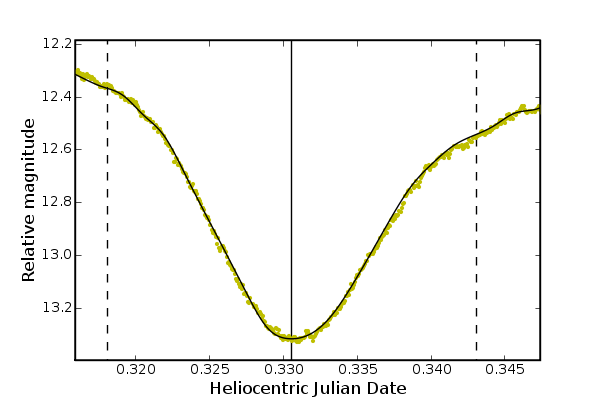
\includegraphics[width=0.85\columnwidth,bb=0 0 600 400]{images/eclipseminimum.png}
 % eclipseminimum.png: 600x400 pixel, 72dpi, 21.17x14.11 cm, bb=0 0 600 400
\caption[Measurement of eclipse minimum]{Plot shows the measured lightcurve(yellow/gray dots), the superimposed smoothing spline (solid black curve) and the measured minimum (solid black vertical line). The broken lines either side of the solid black vertical line are the limits between which the software finds the minimum.}
\label{eclipseminimum}
\end{center}
\end{figure}


See Figure \ref{eclipseminimum}. This is then repeated for all the eclipses. Careful record must be kept of the number of eclipses that occurred after the first eclipse, to ensure no cycle slips occur. Cycle slips will show up as big residuals in the least-squares calculation. See figure \ref{ephemeris}. A value of $N=20$ was used for this particular case. After this has been done for all the available eclipses, the resulting eclipse times and cycle numbers are plotted. Over the timescale of these measurements($\approx$ 30 days), the eclipse times vs cycle number is a straight line. See figure \ref{ephemeris}.

A first order function is then fitted to the eclipse times using least-squares to derive a precise value of the period. I used a parametric least squares adjustment to estimate the period and its standard error. The method is outlined below.

The function to be fitted is written in the following form, $$  v = Ax - l $$ where $x$ contains unknowns, $v$ contain the residuals, $l$ contains the measured values and $A$ contains the coefficients of the unknowns. It can then be shown that the best fit values $x$ are given by $$ x = (A^{T}A)^{-1}A^{T}l $$ where $A^{T}$ denotes the matrix transpose of $A$. 

It can also be shown that the error estimates can be calculate from the following relation, $$ \Sigma_{xx} = \sigma^{2}_{0} \Sigma $$ where $$ \Sigma = (A^{T}A)^{-1} $$ and $$ \sigma^{2}_{0} = \frac{v^{T}v}{n-u} $$ where $n-u$ is the degrees of freedom of the solution. The matrix $ \Sigma_{xx} $ is known as the \textit{variance-covariance} matrix. The diagonals in this matrix contain the variances of the unknowns and the off-diagonal terms contain the covariances.


\begin{figure}
\begin{center}
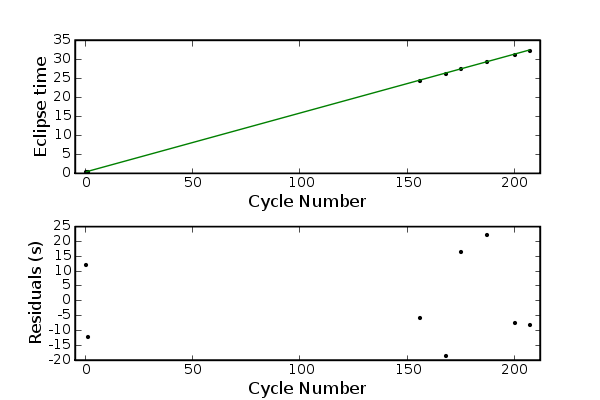
\includegraphics[width=0.85\columnwidth,bb=0 0 600 400]{images/ephemeris.png}
% ephemeris.png: 600x400 pixel, 72dpi, 21.17x14.11 cm, bb=0 0 600 400
\caption[Plot of Eclipse times versus cycle number]{The top plot shows eclipse times vs cycle number and the best fit ephemeris. The bottom plot shows the residuals after the best fit line have been subtracted. The units on the ordinate is seconds}
\label{ephemeris}
\end{center}
\end{figure}


The result from this method gives the period as $$ P = 13351.06 \hspace{4pt}s \pm 0.07 \hspace{4pt}s $$ where all the units are in seconds. See Figure \ref{ephemeris}.  The calculations were made using a program written using the \texttt{Python} programming language and the extension libraries, \texttt{Scipy} and \texttt{Matplotlib}. The spline minimum was calculated using the \texttt{Scipy} function, \texttt{fminbound}.


\section{Flattening of Lightcurves}

\label{flat_section}

\begin{figure}
\begin{center}
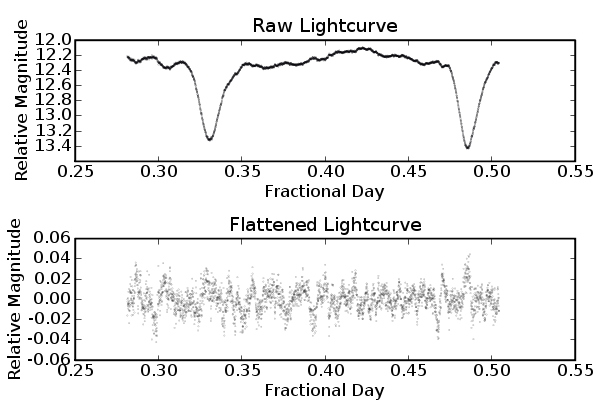
\includegraphics[width=0.85\columnwidth,bb=0 0 600 400]{images/splineandflat.png}
% splineandflat.png: 600x400 pixel, 72dpi, 21.17x14.11 cm, bb=0 0 600 400
\caption{Lightcurve with fitted spline and ``flattened'' lightcurve}
\label{splineandflat}
\end{center}
\end{figure}





The photometric observations were made in order to identify certain periodic phenomena in the brightness of the object. This was done using the standard method of using Fourier analysis techniques. Periodograms of the lightcurves were calculated and the DNOs and lpDNOs were identified as peaks above the noise level. However, since the object undergoes an eclipse approximately every 3.7 hours, large low frequency peaks appear in the periodograms that can suppress low amplitude peaks in the periodogram. See Figure \ref{unflat} for an example. It was therefore decided to try and ``flatten'' the lightcurves in order to remove variations in the brightness profile that are caused by the object's orbit.


It was decided to again use smoothing splines for this operation. However, this path is fraught with danger, since any smoothing operation may inadvertently corrupt the lightcurve and therefore the resulting periodogram. Care was taken to only allow the splines to vary over periods longer than the oscillations being studied. The test was to compare the periodogram of an unsmoothed lightcurve to that of a smoothed lightcurve. The smoothed lightcurve's periodogram should still show the short period variations but not those created by the orbital motion of the binary stars. See Figure \ref{flat} for an example.

\begin{figure}
\begin{center}
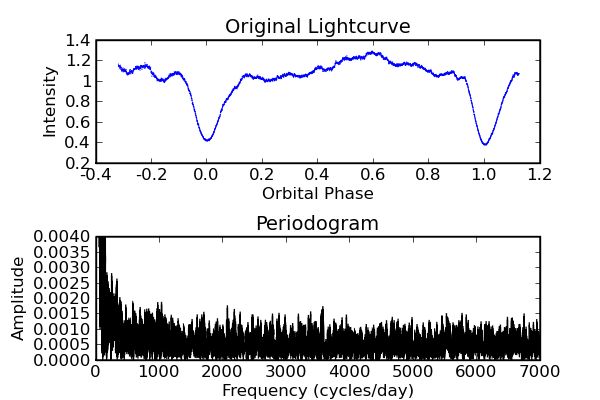
\includegraphics[width=0.85\columnwidth,bb=0 0 600 400]{images/unflattened.png}
 % unflattened.png: 600x400 pixel, 72dpi, 21.17x14.11 cm, bb=0 0 600 400
\caption[Original lightcurve and periodogram]{Plot showing original lightcurve and its periodogram. The periodogram is totally dominated by low frequency noise and no details can be discerned}
\label{unflat}
\end{center}
\end{figure}

\begin{figure}
\begin{center}
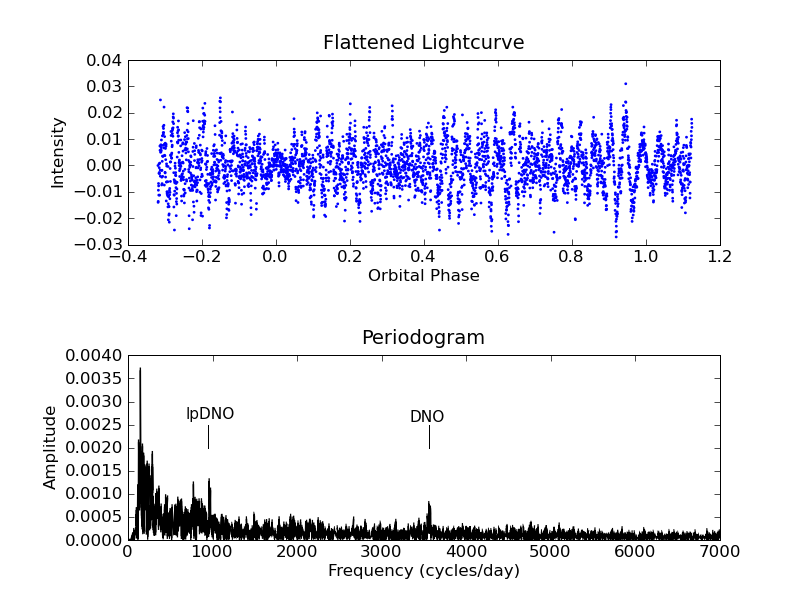
\includegraphics[width=0.85\columnwidth,bb=0 0 600 400]{images/flattened.png}
% flattened.png: 600x400 pixel, 72dpi, 21.17x14.11 cm, bb=0 0 600 400

\caption[Flattened lightcurve and periodogram]{Plot shows the ``flattened'' lightcurve and its associated periodogram. Details in the periodogram can now be identified. Note the DNO peak at $\approx 3600 c/d$ and lpDNO peak at $\approx 1000 c/d$. }
\label{flat}
\end{center}
\end{figure}

The lightcurves were ``flattened'' by calculating a smoothing spline fitting every $N$ points. The spline was then evaluated at the same times the observations were made at. The resulting points obtained from the spline were subtracted from the lightcurve to produce the ``flattened'' lightcurve. Cubic splines were again used for this operation. They were typically fitted to every 40 - 80 points (corresponding to 240 - 480 seconds). See Figure \ref{splineandflat} for an example.


\section{$O-C$ Diagrams}

\label{ominc_section}

\begin{figure}
\begin{center}
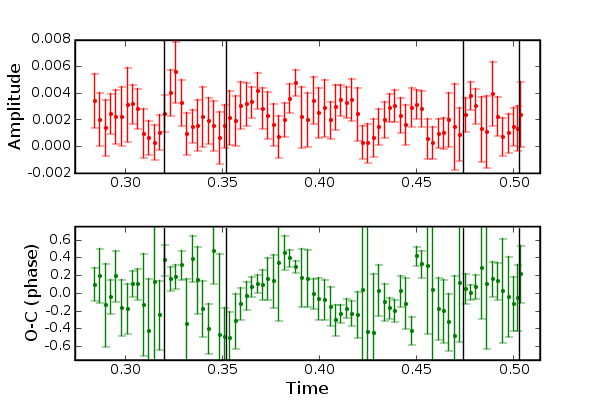
\includegraphics[width=0.85\columnwidth,bb=0 0 600 400]{images/ominc_example.png}
% ominc_example.png: 600x400 pixel, 72dpi, 21.17x14.11 cm, bb=0 0 600 400
\caption[Example of $O-C$ diagram]{$O-C$ diagram of the ``flattened'' version of the lightcurve observed on 16 August 2006. The top plot shows the variation in the amplitude of the  $3559.19\hspace{4pt} c/d$ DNO. The bottom plot shows the variation of the phase of the DNO. The eclipses are marked with double vertical lines. Note wrapping in the phase plot during the first eclipse and immediately before the second eclipse. The diagrams were calculated using $20$ cycles with $50\%$ overlap }
\label{omincexample}
\end{center}
\end{figure}


In order to study the evolution of DNOs, lpDNOs and QPOs, it is necessary to track the changes in their amplitude and phase as a function of time. This was done for this project using the following technique.

The lightcurves were flattened using the techniques described in Section \ref{flat_section} on page \pageref{flat_section}. The periodogram of the flattened lightcurve was then calculated and the frequencies at which the DNO and lpDNO peaks occurred were noted. An $O-C$ diagram was then plotted of the DNO or lpDNO at the frequencies found in the periodogram.

The $O-C$ diagrams used were calculated by fitting a \textit{sine} function to overlapping segments of the lightcurve. The amount of overlap was chosen to be $50\%$, in order to minimise fitting error and to sample the lightcurve at closer intervals. Each segment would typically contain $5$ to $40$ cycles of the variation under inspection. Knowing the sampling rate of the data, the frequency to be studied and the number of cycles to use in the process, it is trivial to calculate the number of data points to use for a segment. The fitting function used for the $O-C$ diagrams were $$y(t) = Acos(2\pi Ft) + Bsin(2\pi Ft)$$ where $$Amplitude =\sqrt{A^{2} + B^{2}} $$ and $$ \phi = arctan(\frac{-B}{A}) $$
The amplitude and phase were then plotted as a function of time. See figure \ref{omincexample}. The fitting was done using the method described in section \ref{ephemeris_section}.

Examination of $O-C$ diagrams may reveal changes in the frequency and amplitude of an oscillation. A change of frequency will show up as ``wrapping'' on the $phase$ vs $time$ plot. An example of this can be seen in figure \ref{omincexample}.

\section{Spectrograms}
\label{spectrogram_section}
A different way of looking at frequency and amplitude changes in a signal is to use a spectrogram. The spectrograms used in this analysis were computed by calculating periodograms of 600s segments of a lightcurve with consecutive segments overlapping by 50\%. The periodograms are then plotted in an image with the vertical axis displaying frequency, the horizontal axis displaying time and the image value displaying amplitude. The time for each periodgram (i.e. column) was calculated by taking the average value of the times in the segment. See figure \ref{trailed_ft_example} for an example. Periodograms were calculated using the algorithm in \cite{kurtz_ft}.

\begin{figure}
 \centering
 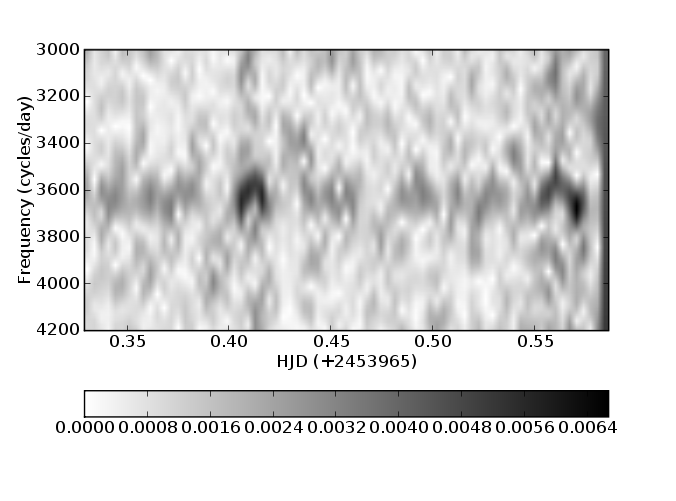
\includegraphics[width = \columnwidth, bb=0 0 600 400]{images/spectrogram_example.png}
 % vel_ew.png: 1179666x1179666 pixel, 0dpi, infxinf cm, bb=0 0 600 400
 \caption{Spectrogram for run S7655. }
 \label{trailed_ft_example}
\end{figure}


\chapter{Spectroscopy}

\label{meth_spec}

\section{Southern African Large Telescope}
\label{SALT}

The Southern African Large Telscope (SALT) is the newest addition to the collection of telescopes operated by the South African Astronomical Observatory (SAAO). The construction have recently been completed and the telescope is currently in its performance verification stage. It already produced its first scientific results \citep{salt_first_science}.

This telescope is the largest single telescope in the southern hemisphere. Its design is based on the Hobby-Eberly Telescope (HET) situated at McDonald Observatory. The unique design of these telescopes allow large telescopes to be built for a fraction of the cost of conventional Altitude-Azimuth (Alt-Az) telescopes. 

The telescope is unconventional in the sense that its instruments are installed in a moving structure called the \texttt{Tracker}. The tracker moves the instruments along a theoretical surface that is concentric with the spherical surface of the main mirror. Therefore in principle, it works in a similar fashion to the Arecibo radio telescope. The tracker is located at a distance of $13.08 \hspace{2pt}m$ from the primary mirror, which is half its radius of curvature. Since the primary mirror is spherical, the tracker houses a spherical aberration corrector (SAC)\citep{dod2000}.

The main mirror consists of 91 hexagonal mirrors made of Astro-Sitall \citep{swiegers}. Each mirror is supported by  actuators. These are used to tip-tilt corrections of the individual mirror segments. The individual segments are also also fitted with capacitive edge sensors, which are used to detect changes in the position of the individual mirrors. The changes can then be corrected. During observation, this is done at $20\hspace{2pt}s$ intervals.

The primary mirror is supported by a steel structure which fixes the altitude the telescopes points at, to $37^{\circ}$. The telescope can only move in azimuth. The telescope can therefore only point to objects in an annulus in the sky at any particular moment. To observe targets outside the annulus, the operators will have to wait for the objects to move into the annulus. Objects can generally be observed twice in an evening. If the objects happen to move across the northern or southern regions of the annulus, they can be observed for longer periods ($\approx$ 4 hours) than when they move overhead from East to West ($\approx $ 1 hour on each side). To observe an object, the telescope will be moved to the appropriate azimuth. The tracker will then be used to follow the object as it tracks across the primary mirror.

Since the telescope cannot be pointed to arbitrary positions on the sky, the observations must be applied for by prospective users, who will send in proposals for their observations. The proposals will be studied by a group of astronomers, who will then appoint priorities for each accepted proposal. The observations will then be scheduled according to visibility of target and priority of observations. \textbf{KRY `N REFERENCE VIR DIE!!!!!!!!!!}.


\section{Robert Stobie Spectrograph}
\label{RSS}

Hier gaan stuff kom van die RSS.



\section{Observations}
\label{spec_obs}


\begin{figure}
\begin{center}
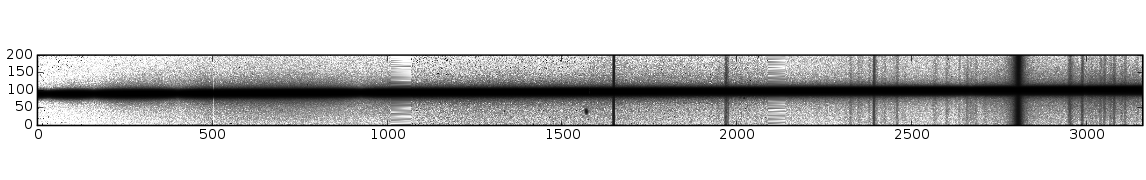
\includegraphics[width=\columnwidth,bb=0 0 600 100]{images/rss_example.png}
% rss_example.png: 1600x1096 pixel, 72dpi, 56.44x38.66 cm, bb=0 0 1600 1096
\caption[Example of spectroscopic exposure.]{Example of spectroscopic exposure. This is an exposure of a spectrophotometric standard star.}
\label{rss_example}
\end{center}
\end{figure}



\section{Reduction of Spectroscopic Observations}
\label{spec_reduce}

The Robert Stobie Spectrograph (RSS) is the first-generation spectrograph fitted to the SALT. It was previously known as the Prime Focus Imaging Spectrograph (PFIS). It is a medium resolution ?? spectrograph with 3 CCD detectors. Each CCD has 2 amplifiers in order to reduce the readout time. A raw SALT RSS FITS file therefore consists of six data blocks and a single header block. In order to extract a spectrum from an image, it is necessary to perform a number of initial operations on the raw FITS file to get the data in a usable form. 

It was decided to perform the spectroscopic reductions separately on each ccd. Knowledge of the relative positions and rotations between the CCD's would therefore not be needed. Each CCD image was separately mosaiced, calibrated, extracted and wavelength calibrated. The three resulting spectra were then joined to form a single spectrum. These steps are outlined below.

The preparation of the images were performed using a script written by the author in the \texttt{Python} language. An example of it can be seen in section \ref{pysalt}. 

\subsection{Mosaicing and Calibration}
\label{calibrate}

Each CCD has 2 amplifiers which will generally have different nominal gain settings at the time the image is read from the CCD device. The different amplifiers will therefore need to be gain corrected separately, each with its own gain value. It was found that using the gain values specified in the FITS header, resulted in an extracted spectrum that exhibited discontinuities across the boundary between different amplifiers as well as between adjacent CCD's. This problem was fixed by calculating the median value of pixels on either side of each boundary and calculating a multiplication factor that will allow the extracted spectrum to be continuous across these boundaries. The gain factors did not need to be absolute since the extracted spectra was later flux calibrated using observations of a spectrophotometric standard star.

Each CCD was then bias corrected using the overscan region. The median value of the overscan region was calculated and subtracted from the CCD image.

The mosaicing of these CCD images was trivial since they do not overlap. The size of the resulting image was known \textit{a priori}. A new empty image was created with dimensions $(R,2C+1)$ where $R$ is number of rows and $C$ is number of columns of each amplifier region. The two amplifier images were then added to the empty image in their correct place. The extra column inserted is the boundary between adjacent amplifiers. This empty column was filled by replacing every empty pixel by the average value of its two adjacent pixels. The bad column on CCD no. 1 was also corrected in this fashion.

Since the flatfield images had a number of saturated pixels, the spectroscopic images could not be corrected for pixel to pixel variations.

The resulting calibrated and mosaiced images were then written to disk in a new FITS file. Selected header entries copied from the primary header unit was added to each output file.

These steps were performed automatically on all raw files using the script shown in section \ref{pysalt}.


\subsection{Spectrum Extraction}
\label{specextract}

The next step in the reduction process was to obtain wavelength- and flux-calibrated spectra from the prepared images. The extraction was done using the popular \texttt{IRAF} package. It was found that automating complex reductions of this nature is made difficult when using the scripting facilities in standard \texttt{IRAF}. Instead, \texttt{Pyraf} scripts were used to automate the spectrum extraction process. The steps followed were obtained from \cite{slitspecIRAF}.

In order to automate the reduction process, an example reduction was made manually to model subsequent reductions on. Since it was decided to separately extract and wavelength calibrate each CCD, 3 manual extractions were made for the EC2117-54 images. There was only a single exposure obtained for EG21, the spectrophotometric standard star. The extraction process for these images were completed manually using the \texttt{apall} task in \texttt{IRAF}.

The steps needed to extract an exposure is as follows,

\begin{itemize}
 \item Locate spectrum on image
 \item Trace spectrum
 \item Specifying spectrum and background windows
 \item Extraction using optimal method
 \item Extracting calibration arcs
 \item Identifying calibration arc lines and wavelength calibration
\end{itemize}

These steps were completed manually for the first exposures on each CCD. The object and background windows were specified in the interactive window of the \texttt{apall} task.

The second step is to trace the spectrum. This is the process of finding the center of the object spectrum along the dispersion direction. This is necessary since, any misalignment in the spectrograph as well as the differential atmospheric refraction for different wavelengths can cause the spectrum to not be perfectly aligned with the pixel rows on the CCD. The image columns are summed along the dispersion direction in multiple steps. For each summed column, the row number of the peak is found. The peak positions as a function of column number is then fitted with a polynomial. This function will then define the center of the spectrum in subsequent reductions.

At this point the spectrum could be extracted from the image. The \texttt{apall} task was used for this purpose. It allows different extraction algorithms to be used. The ``Optimal'' algorithm were used to extract all the spectra. This algorithm weights every pixel according to its noise characteristics. It takes into account Poisson and readout noise. Therefore, pixels with a high signal-to-noise ratio will be given bigger weights. This reduces the amount of noise in the extracted spectrum that is caused by pixels with low signal-to-noise ratio. The details of this algorithm are given in \cite{HorneOpt}.

The calibration arcs were then extracted using the same extraction window as the object spectra.

Subsequent exposures were extracted by using the first as starting point and then refitting the trace. The reductions were done by using the \texttt{Python} script in appendix \ref{spec_extr}.


\subsection{Spectrum Calibration}
\label{spec_cal}

The extracted spectra now needs to be wavelength and flux-calibrated. The wavelength calibration process were done using the \texttt{identify} task in \texttt{IRAF}. This was done for a single arc spectrum. The subsequent arc spectra were wavelength calibrated using the \texttt{reidentify} task. These tasks calculate the dispersion solution for each exposure which were then applied to the object spectra using the \texttt{dispcor} task.

The flux calibration were based upon the spectrum of the spectrophotometric standard star, EG21. The sensitivity function was calculated using the \texttt{sensfunc} task and was applied to the object spectra using the \texttt{calibrate} task. See figures \ref{uncaleg21} and \ref{caleg21}.

The steps followed for these can be found in \cite{slitspecIRAF}.



\begin{figure}
\begin{center}
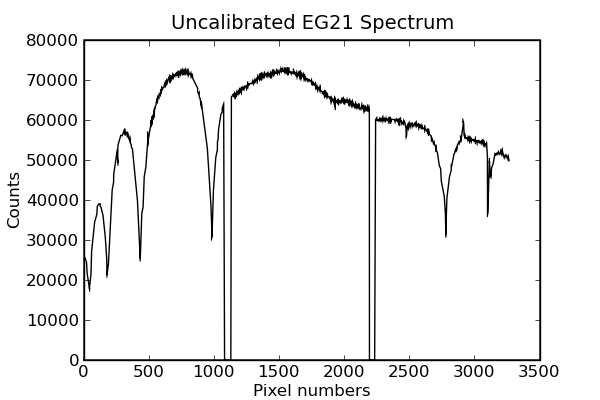
\includegraphics[width=0.9\columnwidth, bb=0 0 600 400]{images/uncalEG21.png}
 % uncalEG21.png: 1179666x1179666 pixel, 0dpi, infxinf cm, bb=0 0 600 400
\caption[Uncalibrated EG21 spectrum]{Uncalibrated EG21 spectrum}
\label{uncaleg21}
\end{center}
\end{figure}

\begin{figure}
\centering
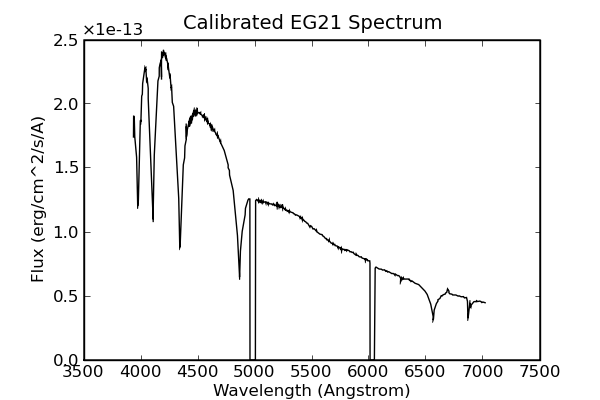
\includegraphics[width=0.9\columnwidth, bb=0 0 600 400]{images/calEG21.png}
\caption[Calibrated EG21 spectrum]{EG21 spectrum after wavelength and flux calibration}
\label{caleg21}
 % uncalEG21.png: 1179666x1179666 pixel, 0dpi, infxinf cm, bb=0 0 600 400
\end{figure}

\begin{figure}
\centering
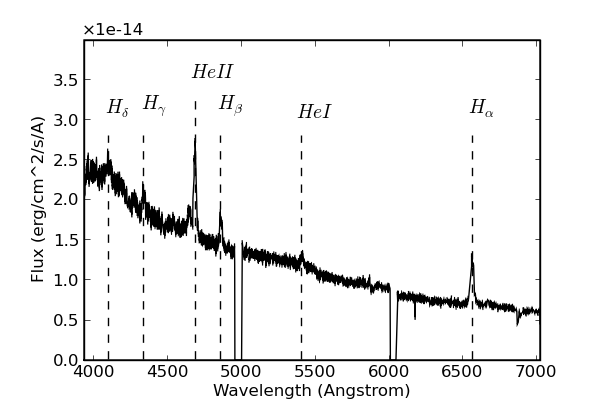
\includegraphics[width=0.9\columnwidth, bb=0 0 600 400]{images/EC2117.png}
\caption[Averaged EC2117 spectrum]{Averaged EC2117 spectrum after wavelength and flux calibration}
\label{avEC2117spec}
 % uncalEG21.png: 1179666x1179666 pixel, 0dpi, infxinf cm, bb=0 0 600 400
\end{figure}

\begin{figure}
\centering
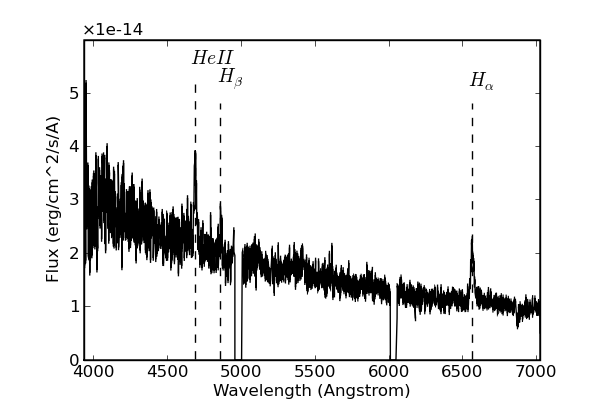
\includegraphics[width=0.9\columnwidth, bb=0 0 600 400]{images/EC0010.png}
\caption[Averaged EC2117 spectrum]{Single EC2117 spectrum after wavelength and flux calibration}
\label{singleEC2117spec}
 % uncalEG21.png: 1179666x1179666 pixel, 0dpi, infxinf cm, bb=0 0 600 400
\end{figure}



